\documentclass[12pt]{article}

% USEPACKAGES
\usepackage[margin=2.5cm]{geometry} % Change border margins.
\usepackage[titles]{tocloft} % Table of Contents, manual add.
\usepackage{mcode} % Load matlab code into LaTeX.
\usepackage[parfill]{parskip} % Removes indents
\usepackage[hidelinks]{hyperref} % Clickable links in PDF.
\usepackage{fancyhdr}
\usepackage{graphicx}
\usepackage{epstopdf}
\usepackage{float}
\usepackage{amsmath,amssymb,amsthm,multirow,algorithm,algorithmic,amsfonts}
\usepackage{gensymb}
\usepackage[square,numbers,comma,sort&compress]{natbib}
\usepackage[titletoc]{appendix}
\usepackage[final]{pdfpages}
\usepackage{afterpage}
\usepackage{mdwlist} % Compact lists (itemize*)
\usepackage{fixltx2e}
\usepackage[table]{xcolor}
\usepackage{madia9}
\usepackage{expl3}


% PAGESTYLE
\pagestyle{plain}

% COMMANDS
\newcommand{\HRule}{\rule{\linewidth}{0.04cm}}
\renewcommand{\abstractname}{{\Large Summary}}
\renewcommand{\cftsecleader}{\cftdotfill{\cftdotsep}}
\setlength{\parskip}{12pt plus8pt minus6pt}

% ENVIRONMENTS
\newenvironment{drawing}


\begin{document}
% Titlepage
\begin{titlepage}
\begin{center}

% Upper part of the page
\textsc{\LARGE Delft University of Technology}\\[0.3cm]
\textsc{\Large Design Synthesis Exercise}\\[0.5cm]

% Title
\HRule \\[0.4cm]
{\Large \bfseries Design of a Controllable Inflatable Aeroshell}\\[0.2cm]
{\Huge \bfseries Project plan}\\[0.2cm]
\HRule \\[1.2cm]

% Image
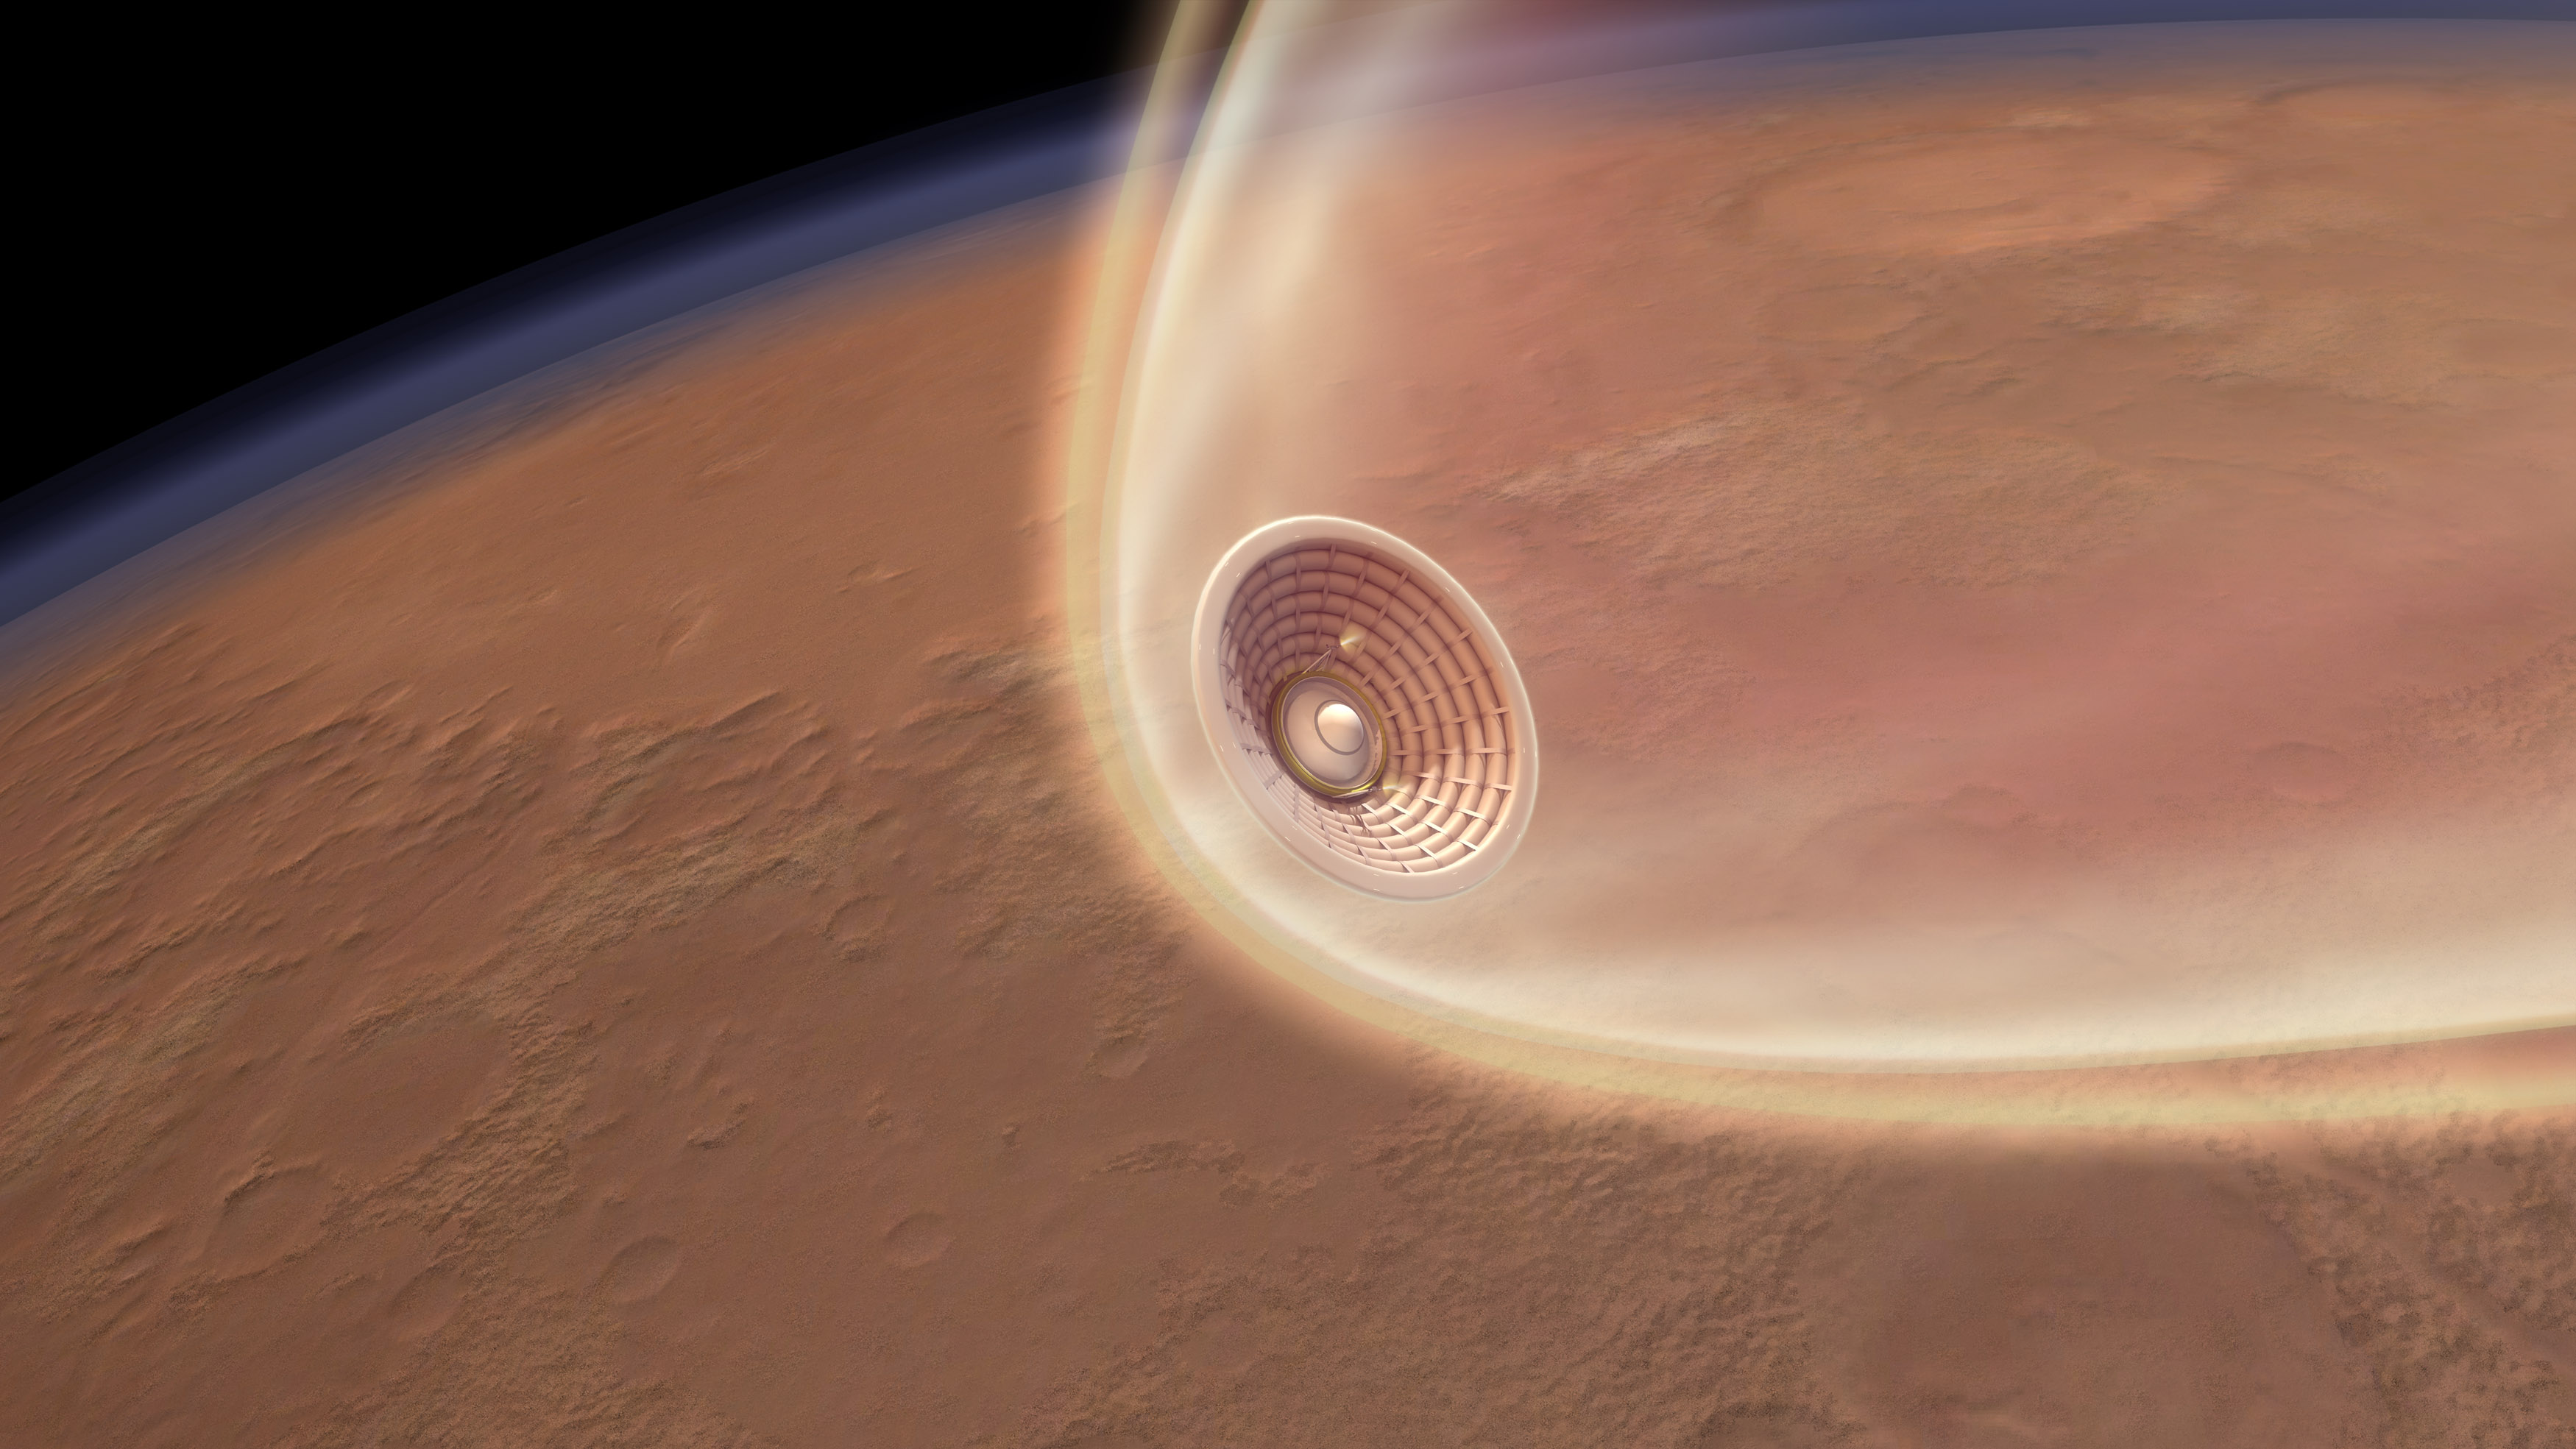
\includegraphics[scale=0.4]{./Titlepage/coverpicture}\\[1cm]

% Author
S. Balasooriyan \\
B. van Dongen \\
D.D. Hage \\
T. Keijzer \\
G. van Koppenhagen \\
L. Mathijssen \\
J. Meulenbeld \\
A. van Oostrum	\\
S. van Schie \\




\vfill

% Date
\begin{large}\today \end{large}

\end{center}
\end{titlepage}
\pagenumbering{roman}
% Preface
\section*{Preface}\label{cha:preface}

\begin{flushright}
	\today
\end{flushright}

Dear Reader,	
\\ [1cm]
A growing interest in manned spaceflight and human exploration of Mars requires a new solution. Conventional, rigid entry solutions require a significant decelerator mass to bring the payload to ground. Inflatable concepts offer significant mass and packaging advantages and their application opens up broad venues for interplanetary human spaceflight. 

This Final Report centres around the analysis and design of a \acrlong{cia} that is capable of bringing two crew members to the Martian surface with a mere $10\%$ decelerator mass fraction within 10 days. Conceptual and preliminary design have shown the feasibility of such a mission with its corresponding economical benefits and reduced ecological footprint by a decreased required number of launches through increased payload-carrying capability.

We would like to acknowledge dr. ir. H.J. Damveld, ir. D. Dolkens and ir. N. Reurings for their guidance and support. Moreover, we would like to thank all other staff members of the Delft University of Technology that have been of assistance.
%This Mid-Term Report is part of the deliverables for the \acrfull{mtr}. It describes the development, verification and validation of the computational tools produced to analyse several possible concepts for a controllable inflatable aeroshell designed for manned spaceflight. In addition to analysing these concepts a trade-off will be made between them to determine which is the most promising. This concept will then be further analysed in the coming period. The goal of this project is to develop an inflatable aeroshell system that can be used for atmospheric entry on Mars and is lighter than the current solutions to this problem.
\\ [1.5cm]
Design Synthesis Exercise Group 02

% Summary
\newpage
\section*{Summary}\label{cha:summary}


Inflatable aeroshell concepts hold the key to what is currently unattainable for interplanetary human spaceflight. In the wake of current \acrfull{nasa} investigations on the feasibility of inflatable decelerators for hypersonic guidable re-entry, this study focuses on Mars entry of a payload mass of at least 9000 [kg] using an inflatable aerodynamic decelerator of at most 1000 [kg]. Such a solution provides a large economical advantage over conventional solutions by maximizing payload-carrying capability through a light-weight device less burdened by launcher size considerations. This Mid-term Report gives an overview of conceptual design activities, comprising aerodynamic, structural, thermal, astrodynamic and control tool development and analysis, leading up to concept selection in a trade-off.
\newline
\newline
To aid in the conceptual analysis, design and selection process and to provide a basis for further design efforts after concept selection in the \acrfull{mtr} a number of tools have been developed with the following purposes:
\begin{itemize}
\item A tool for parametric structural mass modelling
\item A modified Newtonian flow aerodynamic tool for the characterisation of aerodynamic and aerothermal behaviour
\item A thermal model for \acrfull{tps} sizing and analysis
\item An astrodynamic tool with an implemented control system for trajectory control
\end{itemize}

Concepts were selected for trade-off as the outcome of a structured \acrfull{dot} on the basis of concept shape. Shape is chosen to have a leading factor due to its importance in the aerodynamic and trajectory performance, which directly flows down to thermal, structural and control performance. The initial concept selection yielded five concepts for trade-off: a conventional capsule concept and four inflatable concepts, namely stacked toroid, tension cone, trailing ballute and isotensoid configurations. To reflect concept capability of meeting customer demand, the following concept aspects have been evaluated as trade-off criteria: decelerator mass, development risk, vehicle stability and deceleration time.
\newline
\newline
The first trade-off criterion, decelerator mass, is essential since it is highly desirable that payload-carrying capability is maximised. To make full use of the launcher carrying capability, a decrease in decelerator mass allows for an equal increase in payload mass. To this end, structural, thermal and control system mass were estimated as the distinguishing mass components between concepts. 

The lowest structural mass was achieved by the stacked toroid configuration, followed upon closely by the isotensoid, tension cone and trailing ballute configurations (an estimated 110, 168 and 221 \% of stacked toroid structural mass respectively). \acrfull{tps} and control system mass analysis yielded estimates of 100, 84, and 76 \% and 100, 67, and 96 \% of stacked toroid mass for tension cone, trailing ballute and isotensoid configurations respectively. This yields total decelerator masses of 116, 113 and 88 \% of stacked toroid mass, based on weight contributions of 20, 50 and 15 \% by structure, \gls{tps} and control system mass. A mass analysis for the rigid concept showed a decelerator mass well in excess of the imposed maximum 1000 [kg], 2945 [kg] for thermal and structural mass alone.
\newline
\newline
The second trade-off criterion, development risk, is essential since concepts with a low \acrfull{trl} incur higher schedule and cost risks. The tried-and-true rigid solution thereby has \gls{trl} 9, while inflatable concepts are notably less explored. A recent surge in interest in inflatable concepts by \gls{nasa} and a consistent development program has brought the stacked toroid configuration to \gls{trl} 7. The other three inflatable concepts are less explored, having only undergone a selected set of tests and research and hence designated \gls{trl} 4. The trailing ballute concept is deemed to have a higher development risk still, by its only feasible control option being a relatively underdeveloped one, namely morphing, reflected by \gls{trl} 2.
\newline
\newline
The third trade-off criterion, deceleration time, is evaluated as a shorter entry time is desirable. As ground operations are to be maintained at fully capacity during entry, a shortening of entry time will alleviate costs incurred. Moreover, physical taxation of human payload is decreased as deceleration time is decreased.  A decreased deceleration time is obtained by better controlability of the spacecraft. To this end, concepts were evaluated for their performance in lift to drag ratio. The rigid concept was found to be able to provide a relatively high lift to drag ratio which consequently will result in short deceleration time. The stacked toroid, tension cone and ballute concept were found to provide an adequate value and finally the isotensoid deceleration performance was found to be poor in this trade-off criteria.
\newline
\newline
It is preferable that concepts are stable, since a stable vehicle will counteract perturbations to move back to its equilibrium condition and its intended trajectory. To this end, static stability was investigated by aerodynamic analysis. Stacked toroid, tension cone and ballute were found to be stable; the rigid concept is neutrally stable and the isotensoid is unstable. The first three therefore perform well, the rigid concept performs adequately and performance of the isotensoid is deficient for the fourth and final trade-off criterion.
\newline
\newline
On the basis of the analysis presented in this Mid-Term Report, design options and their prospective advantages and disadvantages are presented to the customer at the \gls{mtr}. Hereafter dialogue is entered to yield a final concept for preliminary design that satisfies customer demands. The next phase then commences with a more detailed analysis and design of the selected concepts, aided by tool enhancement. This phase entails a more refined orbit optimization, aerodynamic shape determination and structural and \gls{tps} design and sizing. A structured approach to this next phase is facilitated by breaking down future work, resource allocation and is aided by an interface definition given in this report to define the interaction of subsystems within the design process.

% Table of contents
\newpage
\tableofcontents
\addtocontents{toc}{\protect\contentsline {section}{Preface}{i}{}}
\addtocontents{toc}{\protect\contentsline {section}{Summary}{ii}{}}
\addtocontents{toc}{\protect\contentsline {section}{List of Symbols}{iv}{}}



% Chapters
\newpage
\pagenumbering{arabic}
\section{Introduction}
\label{cha:introduction}
Before human interplanetary spaceflight can be achieved technological gains have to be made in several fields. One of these fields comprises hypersonic deceleration systems. Significant weight gains are expected to be possible by using inflatable aeroshells. However, the development of a controllable inflatable aeroshell is very complex and consists of many different disciplines. To reduce the complexity of designing such a system first a \acrfull{pp} was made. Following that a \acrfull{br} was produced, in order to survey the current technology state and knowledge on this subject. Now a \acrfull{mtr} report is made in order to perform a concept trade-off. 

The purpose of this report is to present several concepts for a controllable inflatable aeroshell and to determine which concept is best suited for performing the design mission. First the group organisation for the period between the \acrlong{mtr} and \acrlong{fr} is discussed in chapter \ref{ch:wdd}, including individual and group tasks and work packages. A \acrfull{wbs} is made, together with a \acrfull{wfd} and Gantt chart. Secondly the approach with respect to sustainable development is presented in chapter \ref{ch:sustain}. Thirdly the \glspl{dot} are used in chapter \ref{ch:options} to generate several system concepts. These concepts will be analysed with tools from several different disciplines. These consist of an astrodynamics \& control tool, as well as tools for concept mass estimation, aerodynamical characteristics and thermodynamic behaviour. The development, verification, validation of these tools is discussed in chapters \ref{ch:astrocontrol}, \ref{ch:strucmass}, \ref{ch:aero_analysis} and \ref{ch:thermtool} respectively. These chapters also show the results obtained from analysing the proposed system concepts. After the tool development and concept analysis the risk inherent to each system concept is considered in chapter \ref{ch:riskestimation}. This will be done by making a risk map for each concept. Finally the concept trade-off will be performed in chapter \ref{ch:tradeoff}, based on results of the analyses conducted in the previous chapters. The result of this is a complete trade-off matrix, after which the customer will be able to select the preferred concept based on the weights they attach to each trade-off criterion.
\newpage
\section{Chapter one}\label{cha:chapter_one}

\subsection{Sub chapter}\label{par:sub_chapter}
\input{./Chapter_one/Sub_chapter}

\begin{figure}[H]
\centering
\includemedia[
width=400pt ,height=0.4\linewidth,
activate=pageopen,3Dmenu,
]{}{./Figure/frontlandinggear.u3d}
\caption{Front landing gear 3d movable model.}\label{3dm:awesome2}
\end{figure}
\newpage
\section{Conclusion}\label{cha:conclusion}

\subsection{Requirements}
In this section the top-level requiremets are stated. They can be found in table \ref{tab:requirements}.

\begin{table}[H]
	\caption {Requirement}
    \begin{tabular}{|l|l|}
    \hline
    Code          & Description                                                                                                      \\ \hline
    CIA-Sys-A01-1 & The re-entry vehicle shall be able to cope with an entry velocity of seven kilometers per second.                \\ \hline
    CIA-Sys-A01-2 & The inflated aeroshall shall have a maximum diameter of 12 meters.                                               \\ \hline
    CIA-Sys-A01-3 & The diameter of the launcher fairing shall be 5 meters.                                                          \\ \hline
    CIA-Sys-A01-4 & The maximum entry mass of the re-entry vehicle shall be 10,00 kilograms.                                         \\ \hline
    CIA-Sys-A01-5 & The hypersonic deceleration system mass shall not be havier than ten percent of the total re-entry vehicle mass. \\ \hline
    CIA-Sys-A01-6 & The control system shall have a maximum failure probability of 5.0e-4.                                           \\ \hline
    CIA-Sys-A01-7 & The maximum allowable loads on the re-entry vehicle shall be 3 earth g's in each axis                            \\ \hline
    CIA-Sys-A01-8 & The re-entry vehicle shall have a maximal aerobraking duration of ten days.                                      \\ \hline
    \end{tabular}
    \label{tab:requirements}
\end{table}



\subsection{System description}


% Bibliography
\newpage
\bibliography{./Bibliography/Bibliography}
\bibliographystyle{ieeetr}
% Appendix
\newpage
\appendix
\section{Project Gantt Chart}

\begin{sidewaysfigure}[ht]
    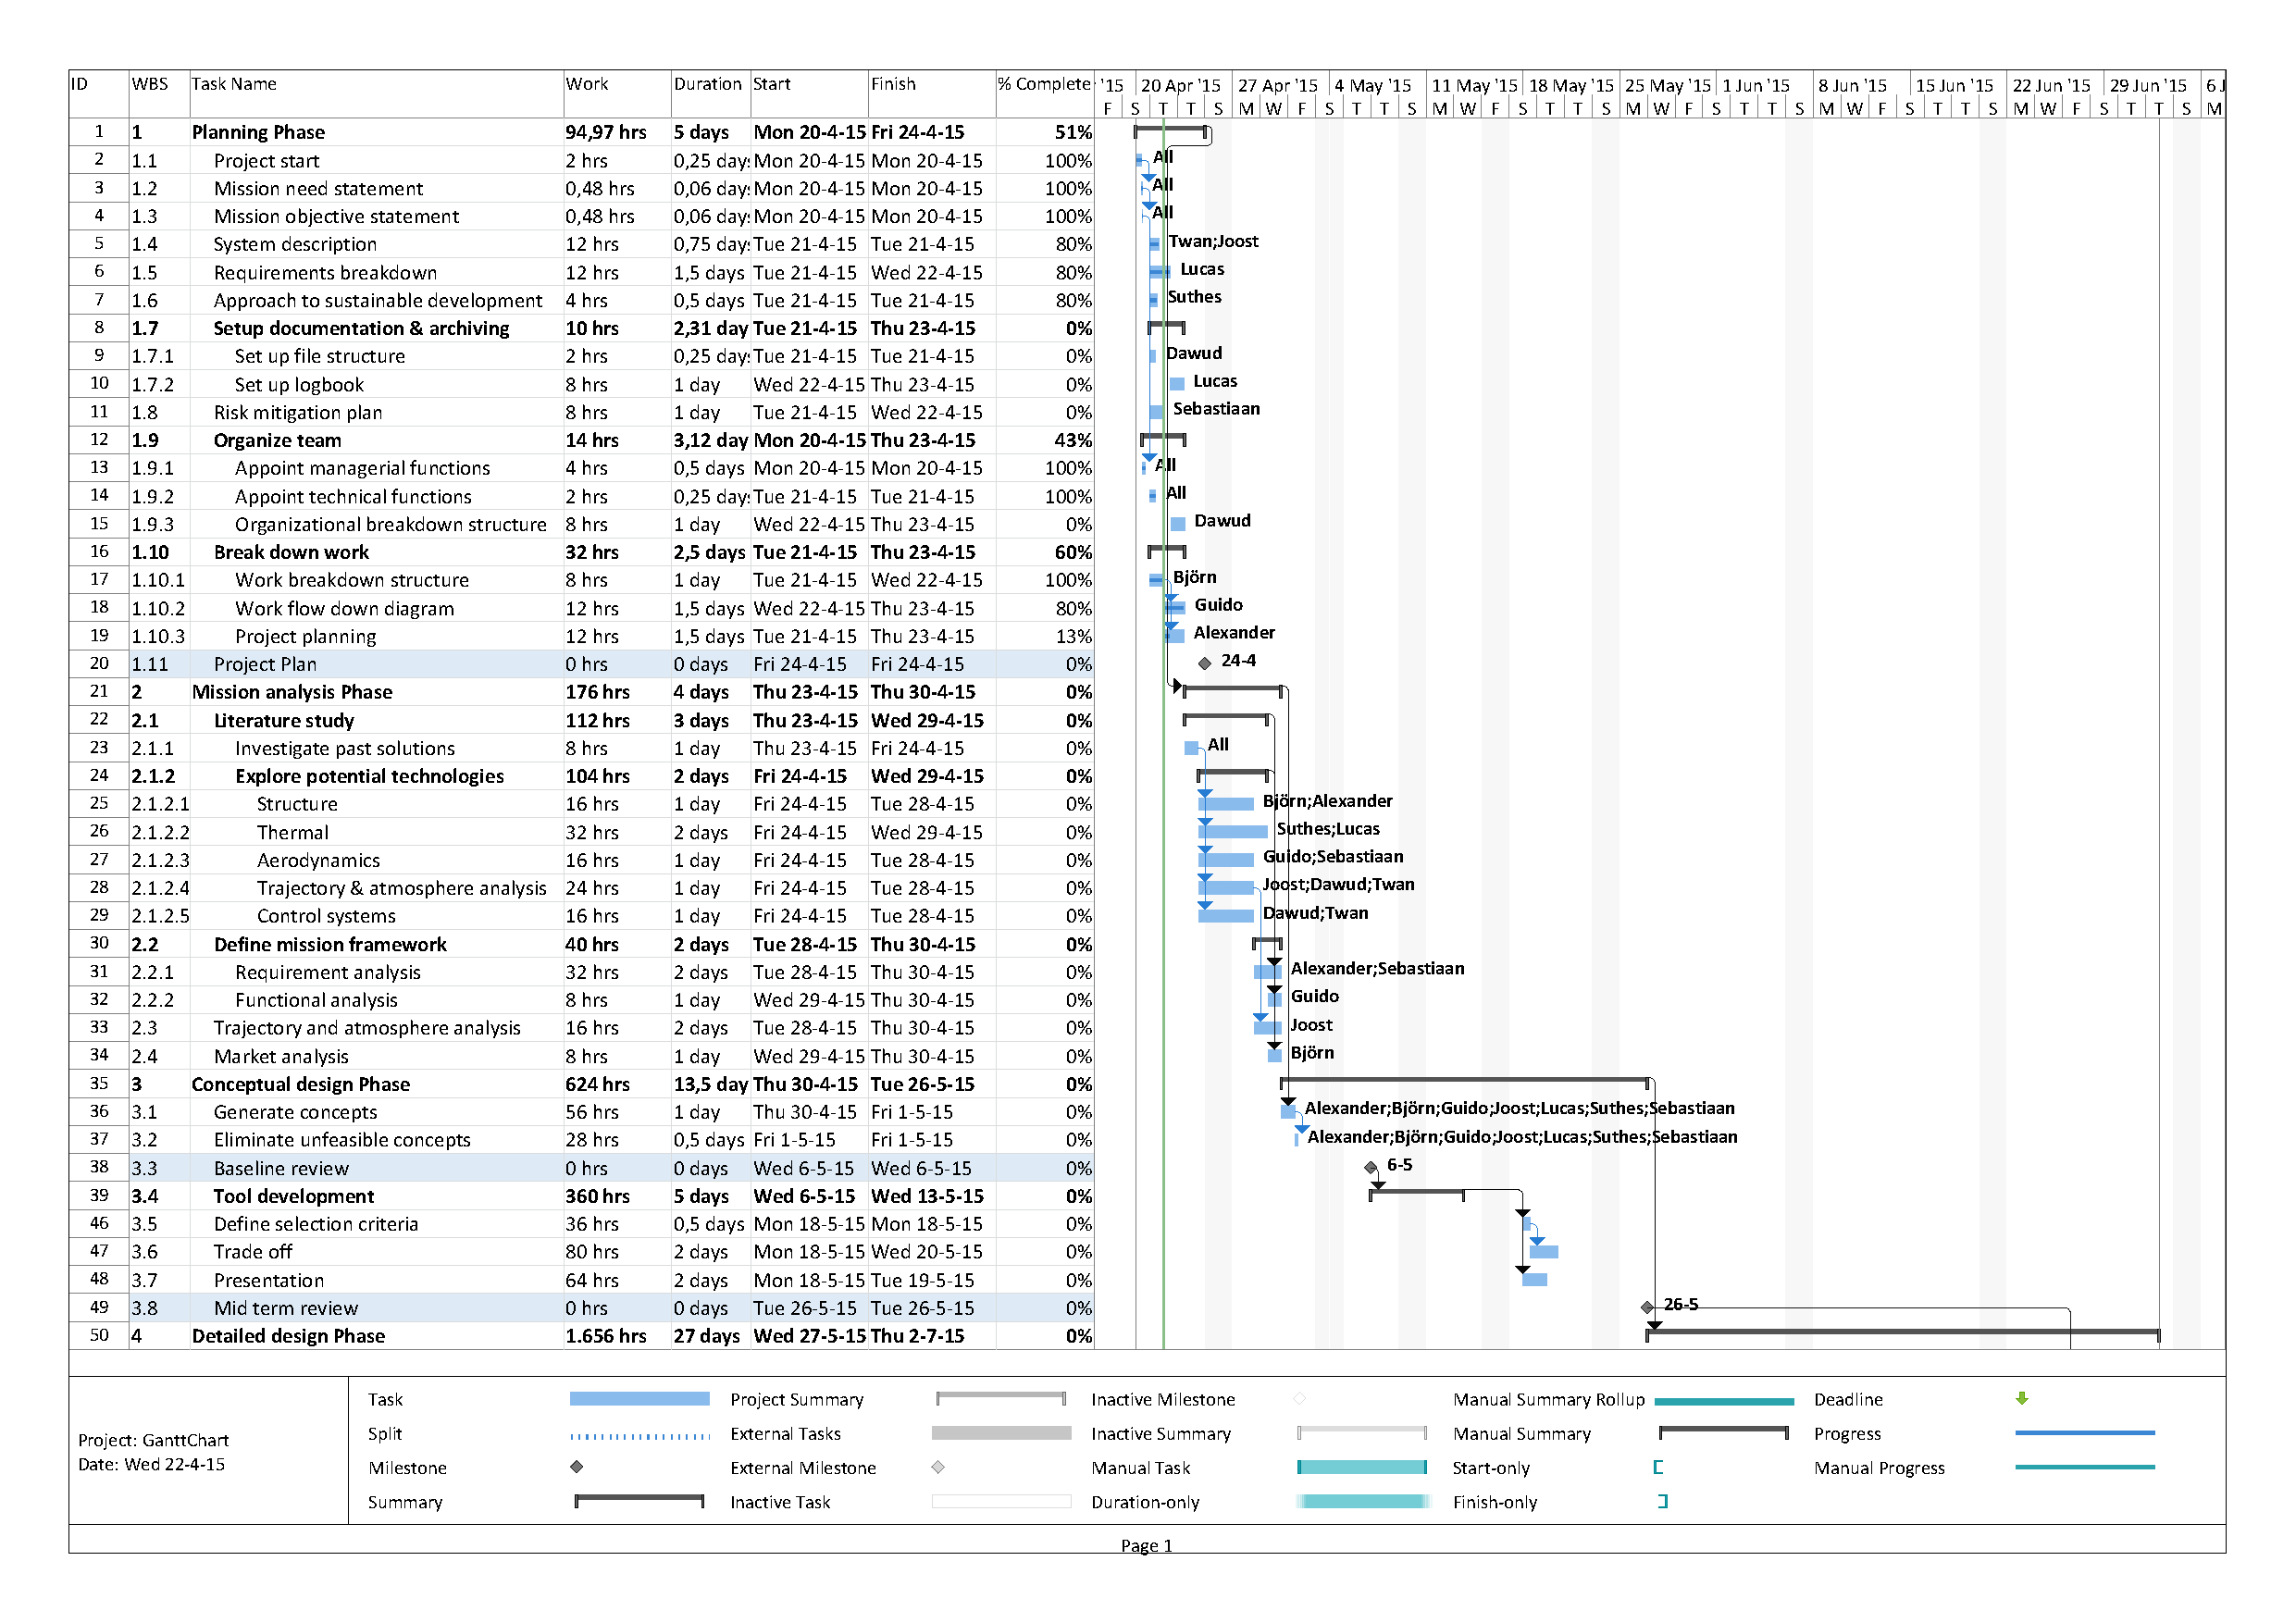
\includegraphics[scale=0.9]{Figure/GanttChart.pdf}
    \caption{Project planning}
    \label{fig:GanttChart}
\end{sidewaysfigure}

\begin{sidewaysfigure}[ht]
    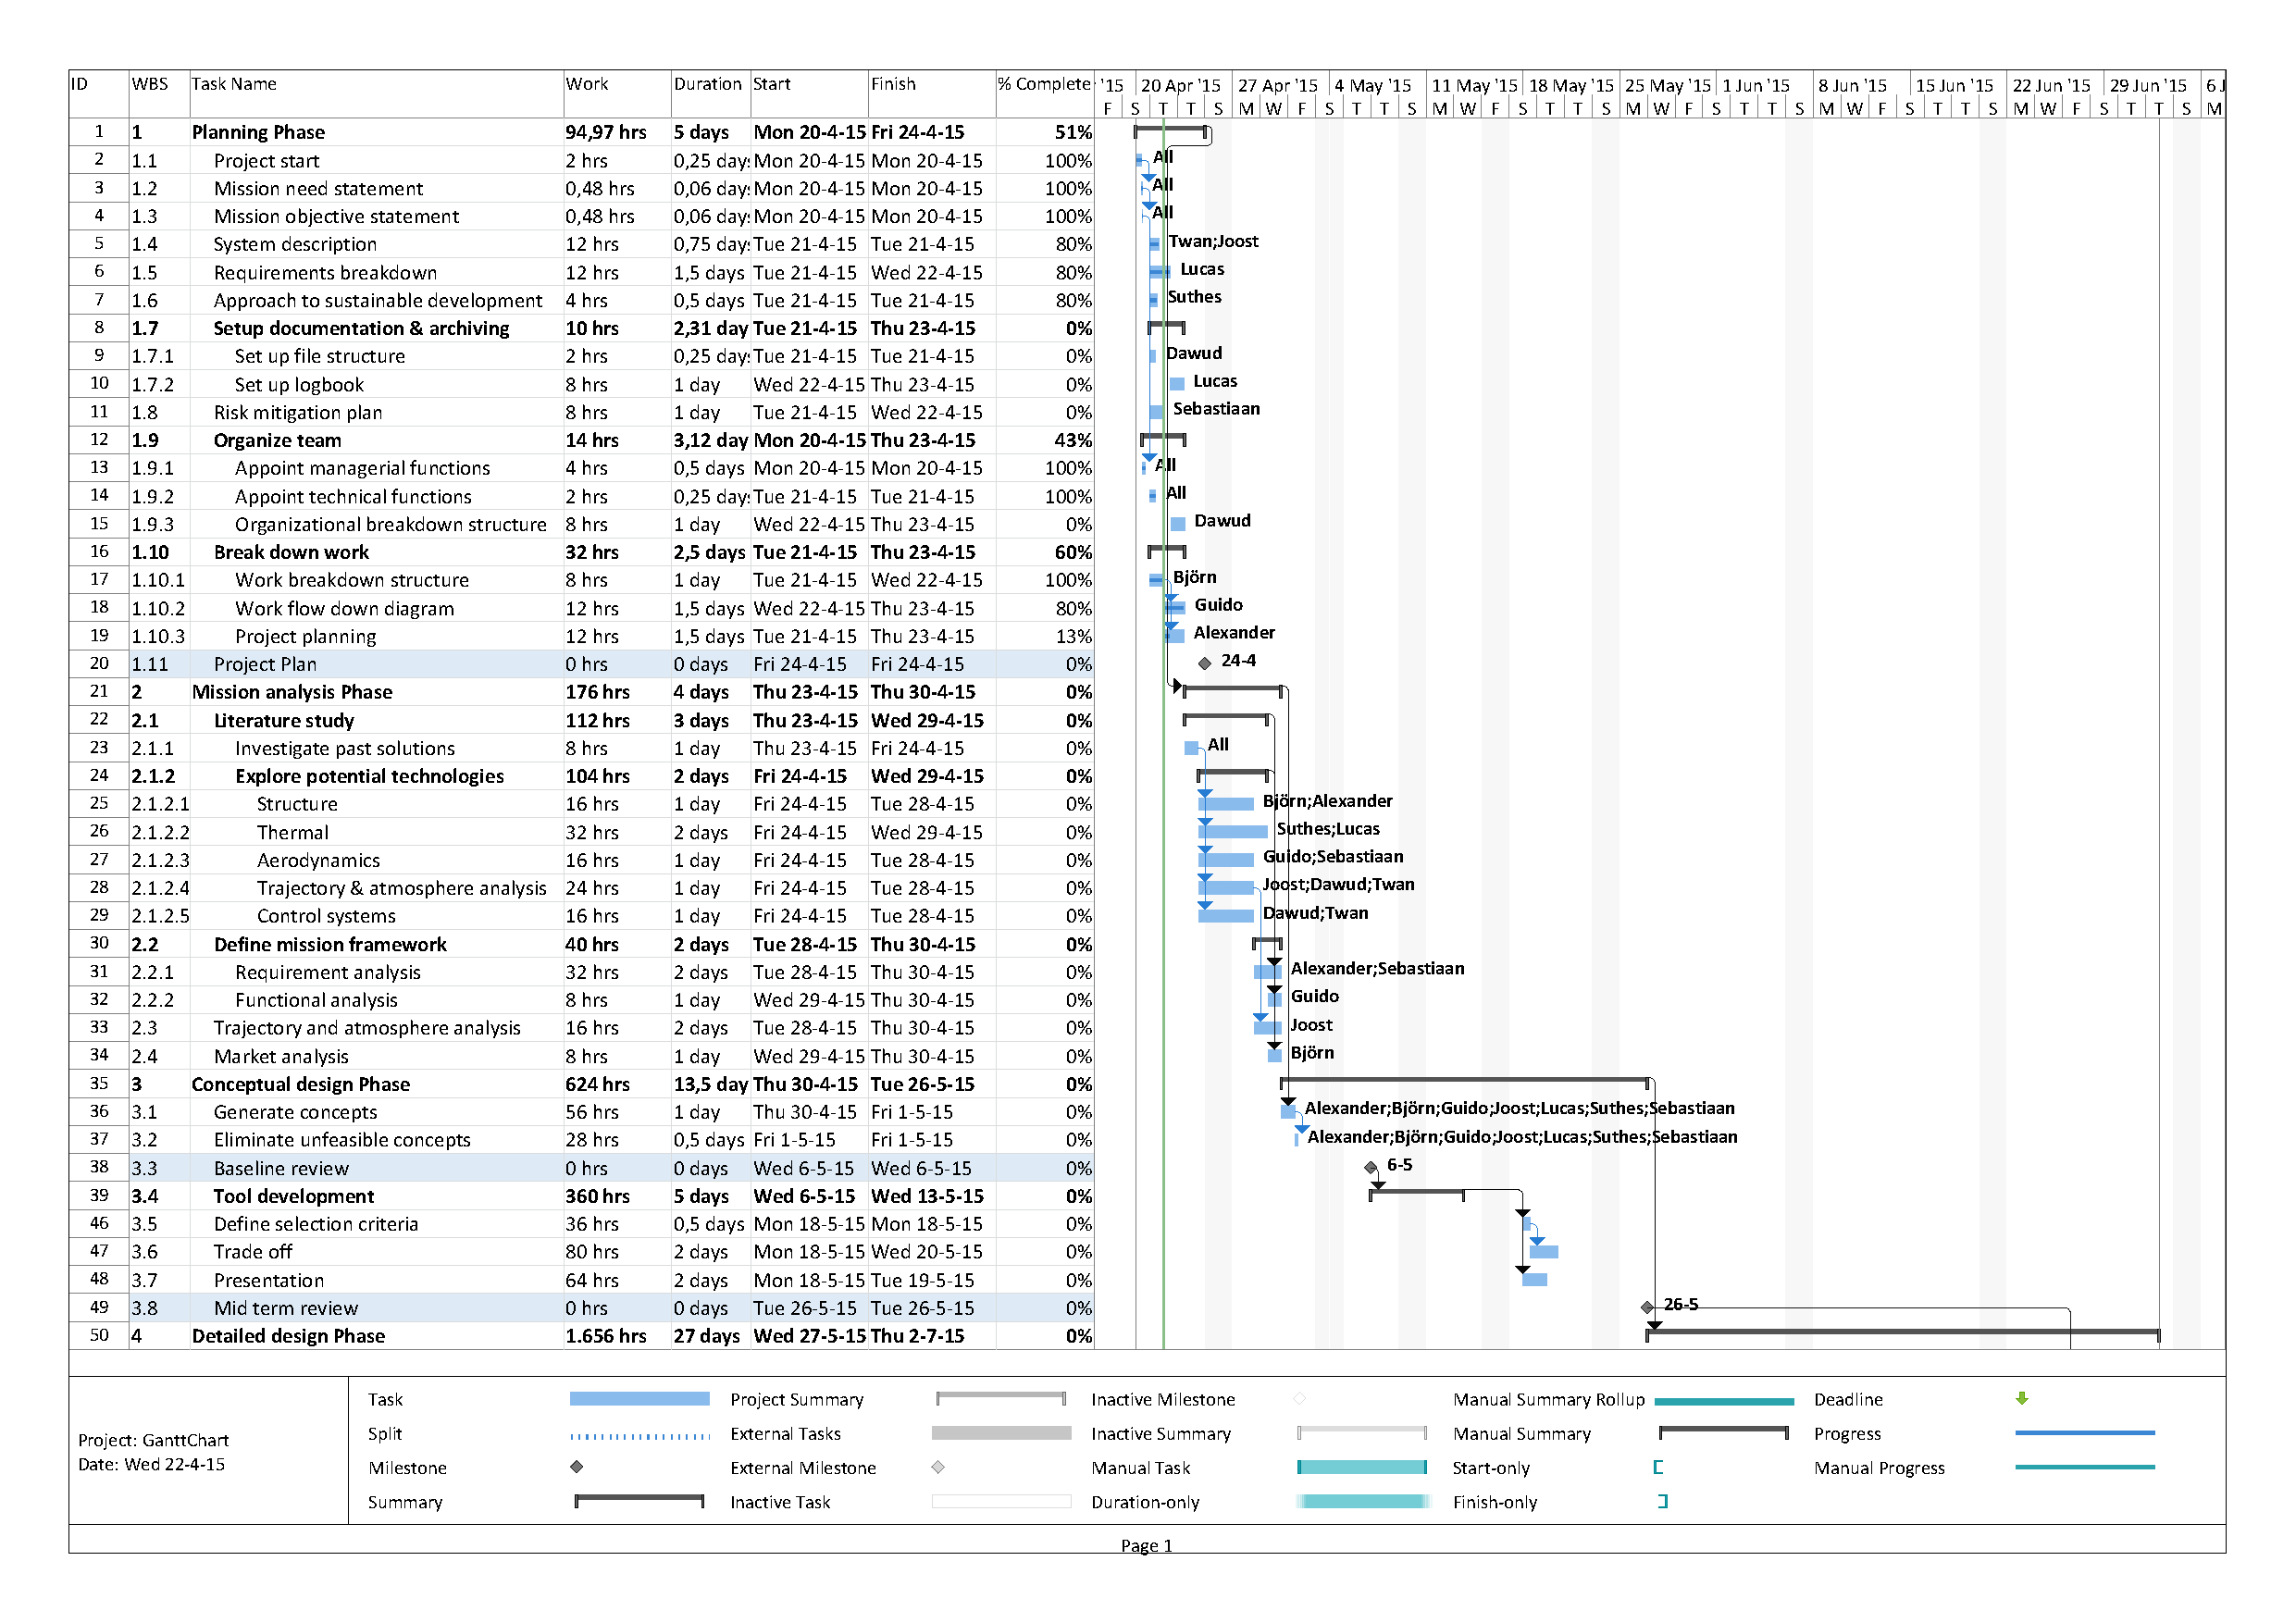
\includegraphics[scale=0.9]{Figure/GanttChart.pdf}
    \caption{Project planning}
\end{sidewaysfigure}

% List of symbols
\newpage
\section*{List of Symbols}\label{cha:listofsymbols}
\begin{table}[h]
\centering
\begin{tabular}{l p{320pt} l}
Symbol & Description & Dimension\\
\hline
\hline
$a$ & Speed of sound & $m/s$\\
\hline
$A$ & Aspect ratio & $-$\\
\hline
$\alpha$ & Angle of attack & $\degree$\\
\hline
\end{tabular}
\end{table}
\end{document}